\chapter{Methode}
For this report, we created a python simulation to simulate the data diffusion and the seed selection. We utilized the Pycx libraries to create the GUI, and applied the R-mat generator to create the different network.

\section{PyCx}
Pycx an librarie that help python to generate an GUI\cite{Pycx}. The pycx have a clear structure, initialize, observe and update. The initialize part, the graph is generated, the starter seed is found and the position to the graph is generated. The observe part is where python generate graphic for our simulation. for each step, the observe is called to generate a new frame. the update section i called every step, for our program, the diffusion is calculated as each step we can see how the data is diffused. The simulation allowe the information and data to be displayed 


\section{R-mat}
One problem during graph analysation and calculation is finding suiteble graphs to analyse. Generate graphs with desirede properties is not easdy to do. One solution proposed by Deeeoayan et al is to use the "recursive matrix" or R-mat model. The R-mat model generates graph with only a few parameters, the generated graph will naturally have the small world propertie and follows the laws of normal graphs, and have a quick generation speed\cite{Rmat2004}. The R-mat models goal is to generate graphs that matches the degree distribution, exhibits a " community " structure and have a small diameter and mathces other criteria.\cite{Rmat2004}.

The R-mat generater generates sociall network with the community structure. The different probability for the four partition is :$A=0.57$,$B=0.19$,$C=0.19$,$D = 1-A-B-C = 0.05$. These different probability was used by GRAPH500[CITATION NEEDED]. The R-mat generated three different adjacency matrices of different size.


The algorithm to generate such a recursive matrix is as follow: The idea is to partition the adjacency matrix into four equally sized part branded A,B,C,D, like shown in Figure\ref{fig:flipDiagonal}. The adjacency matrix starts by having all element set to 0. Each new edge is "droped" onto the adjacency matrix. Which section the edge would be placed in, is choosen randomly. Each section have a probability of $\it{a, b, c, d}$, and $a + b + c + d = 1$. After a section is choosen, the partion that was choosen is partitioned again. This continoues until the choosen section is a 1x1 square and the edge is dropped there. 
\begin{figure}
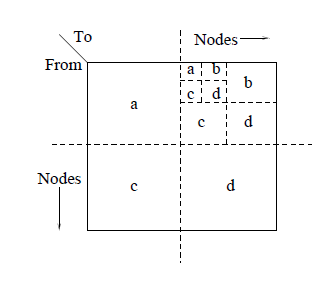
\includegraphics{Rmat}
\caption{The R-mat model}
\label{fig:Rmat}
\end{figure}

From the algorithm, we can see that the R-mat generator is capable to generate graphs with total numbers of node $ \it{V} = 2^x$. Since the algorithm partitioned the matrix into four part. This is approach would only generate a directed graph. To generate undirected graph, $b = c$ and the adjacenmcy matrix must make a "copy flip" on the diagonal elements, like FIgure \ref{fig:flipDiagonal}. 

\begin{wrapfigure}{r}{0.5\textwidth}
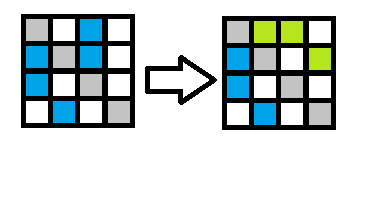
\includegraphics{flip_matrix}
\caption{How the adacency matrix is fliped on the diagonal}
\label{fig:flipDiagonal}
\end{wrapfigure}


\section{Adjacency matrices to graphs}
For this report, four different sized adjacency matrix was created. One of the restriction to the R-mat generator is that the size of the adjacency matrix have to be $2^n$. This resulted in that our adjacency matrix was originaly of the size, $128 \times 128, 512 \times 512 and 1024 \times 1024$. The resulted graphs had multiple singletons and unconnected nodes, for the sake of the simulation, those nodes were discarded and resultede in a graph with 75 nodes and 307 edges, 287 nodes with 2415 edges and 617 nodes and 8374 edges. This was not supprising considere that for a larger graph, those singletons would most likely result in the outer perifier and small community.

\section{The algorithm}
The simulation creates an social network by reading from the adjacency matrix. We implemented 4 different algorithm. The greedy algorith, the degree algorithm, random algorithm, and a independent greedy algorithm. The algorithm implemented, finds the $\it{k}$ vertecies to be the starter nodes. $\it{k}$ is [1,2,  $\dots$ 20]. This is to be able to see how teh size of the starting nodes affect the coverage. For each $\it{k}$, the simulation applies the diffusion for 50 times. This is to finde the mean coverage to remove the randomness 

The greedy algorithms finds the most influential nodes in relation with the other previous picked seeds. The algorithm starts by finding the most influential nodes $s_1$ from the entire graph $\it{G}$, in this instance, k=1. The most influential node is found by just choosing a node and see how much spread it will result in, the value is stored with the node, and after the entire G is itterated over, the node with the highest value is choosen. Then the algorithm stores the node in $\it{S}$ and applies data diffusion and stores the effect this runs had. The next run, k=2 and the greedy algorithm finds the most influential node $s_2$ where $s_2 \neq s_1$ and $s_2 +s_1 = maxCoverage$. This is repeated until k=20. The new run, the seed selection will keep the previous selected seed and during the finding maximum coverage phase, the previous choosen seed will have impact on the run.

The degree algorithm chooses the vertex with the highest degree. Unlike the greedy algorithm. The degree algorithm just finds the vertices with the highest degree. The algorithm chooses $s_1, s_2 \dot 2_k$ from $\it{G}$ that have the highest degree. One of the problem would be that hihger degree nodes would often be connected to each other, the community struckture that was mentioned in previous section. The degree histogram shows us that there are very few high degree node, while having more low degree nodes.

The random algorithm picks random vertices as the starter nodes. This is the simplest algorithm, where each runs, a new random node is added to the set $\it{S}$. Then the diffusion is applied. 

